\ExamPart{Trắc nghiệm đúng sai}{2}{Thí sinh trả lời từ câu 1 đến câu 2. Trong mỗi ý a), b), c), d) ở mỗi câu học sinh chọn đúng hoặc sai.}

\NQuestion Cho đồ thị hàm số $y=f(x)$ như hình vẽ dưới đây.
\begin{center}
    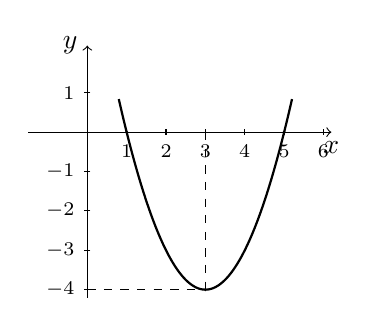
\begin{tikzpicture}[scale=0.5]
    \draw[->] (-1.5,0) -- (6.2,0) node[below] {$x$};
    \draw[->] (0,-4.2) -- (0,2.2) node[left] {$y$};
    \foreach \x in {1,2,3,4,5,6}
      \draw (\x,0.08)--(\x,-0.08) node[below] {\scriptsize $\x$};
    \foreach \y in {-4,-3,-2,-1,1}
      \draw (0.08,\y)--(-0.08,\y) node[left] {\scriptsize $\y$};
    \draw[smooth, samples=200, domain=0.8:5.2, thick] plot (\x, {(\x-3)^2-4});
    \fill (1,0) circle (1.2pt);
    \fill (5,0) circle (1.2pt);
    \fill (3,-4) circle (1.2pt);
    \draw[dashed] (3,0)--(3,-4);
    \draw[dashed] (0,-4)--(3,-4);
\end{tikzpicture}

\end{center}
Xét các khẳng định sau:
\begin{SubQuestions}
  \TFItem{true}{Đồ thị cắt trục hoành tại hai điểm có hoành độ là $1$ và $5$.}
  \TFItem{true}{Trục đối xứng của parabol là đường thẳng $x=3$.}
  \TFItem{false}{Giá trị nhỏ nhất của hàm số bằng $-5$.}
  \TFItem{true}{Bất phương trình $f(x)<0$ có tập nghiệm là $(1;5)$.}
\end{SubQuestions}
\SolutionBlock{Từ đồ thị, parabol mở lên, có hai nghiệm là $1$ và $5$, trục đối xứng là $x=3$, đỉnh có tung độ $-4$, nên ý a), b), d) đúng và ý c) sai.}

\NQuestion Một lớp học có $18$ học sinh nam và $12$ học sinh nữ. Xét các khẳng định sau:
\begin{SubQuestions}
  \TFItem{true}{Số cách chọn ngẫu nhiên $1$ lớp trưởng là $30$.}
  \TFItem{true}{Số cách chọn $1$ nam và $1$ nữ tham gia văn nghệ là $216$.}
  \TFItem{false}{Số cách chọn $2$ học sinh bất kỳ là $30\cdot29$.}
  \TFItem{true}{Số cách chọn một tổ gồm $1$ tổ trưởng và $1$ tổ phó từ $30$ học sinh là $30\cdot29$.}
\end{SubQuestions}
\SolutionBlock{\begin{itemize}[leftmargin=1.5em]
\item Chọn $1$ lớp trưởng từ $30$ học sinh có $30$ cách.
\item Chọn $1$ nam và $1$ nữ có $18\cdot12=216$ cách.
\item Chọn $2$ học sinh bất kỳ phải là $C_{30}^2$, không phải $30\cdot29$.
\item Chọn $1$ tổ trưởng và $1$ tổ phó là hai vị trí khác nhau nên có $30\cdot29$ cách.
\end{itemize}}
